% #############################################################################
% This is Chapter 2
% !TEX root = ../main.tex
% #############################################################################
% Change the Name of the Chapter i the following line
\fancychapter{Fundamental Concepts}
\cleardoublepage
% The following line allows to ref this chapter
\label{chap:back}

This chapter introduces the fundamental technical concepts and architectures underlying open-vocabulary referring segmentation systems.

% #############################################################################
\section{Neural Networks and Deep Learning}

Neural networks form the foundation of modern deep learning systems, providing the computational framework for learning complex patterns from data. The perceptron represents the simplest form of artificial neural network, consisting of a single computational unit that performs a linear combination of inputs followed by a nonlinear activation function, as illustrated in Figure~\ref{fig:perceptron}. For a perceptron with $N$ input features $\mathbf{x} = [x_1, x_2, \ldots, x_N]^T$, the output $y$ is computed as:

\begin{equation}
y = f(\mathbf{w}^T\mathbf{x} + b),
\end{equation}

where $\mathbf{w} = [w_1, w_2, \ldots, w_N]^T$ represents the weight vector, $b$ is the bias term, and $f(\cdot)$ denotes the activation function. This can be expanded as:

\begin{equation}
y = f\left(\sum_{i=1}^{N} w_i x_i + b\right).
\end{equation}

The activation function $f(\cdot)$ introduces nonlinearity into the model, enabling the perceptron to learn complex decision boundaries. Common activation functions include the sigmoid function $f(z) = \frac{1}{1 + e^{-z}}$, the hyperbolic tangent $f(z) = \tanh(z)$, and the rectified linear unit (ReLU) $f(z) = \max(0, z)$.

Multi-layer perceptrons extend the single perceptron by connecting multiple layers of neurons in a feedforward architecture, as shown in Figure~\ref{fig:mlp}. For a neural network with $L$ layers, where layer $l$ contains $n_l$ neurons, the forward propagation process computes:

\begin{equation}
\mathbf{a}^{(l)} = f^{(l)}\left(\mathbf{W}^{(l)}\mathbf{a}^{(l-1)} + \mathbf{b}^{(l)}\right),
\end{equation}

where $\mathbf{a}^{(l)}$ represents the activation vector of layer $l$, $\mathbf{W}^{(l)} \in \mathbb{R}^{n_l \times n_{l-1}}$ is the weight matrix connecting layers $l-1$ and $l$, $\mathbf{b}^{(l)} \in \mathbb{R}^{n_l}$ is the bias vector, and $f^{(l)}(\cdot)$ is the activation function for layer $l$. The universal approximation theorem demonstrates that multi-layer perceptrons with sufficient hidden units can approximate any continuous function on compact subsets of $\mathbb{R}^n$, providing the theoretical foundation for their expressiveness.

Neural networks are trained through gradient-based optimization methods that minimize a loss function $\mathcal{L}(\theta)$, where $\theta$ represents all learnable parameters. The loss function quantifies the difference between predicted outputs and ground truth targets, such as the mean squared error for regression tasks:

\begin{equation}
\mathcal{L}(\theta) = \frac{1}{n}\sum_{i=1}^{n}(y_i - \hat{y}_i)^2,
\end{equation}

where $n$ is the number of training samples, $y_i$ are the true labels, and $\hat{y}_i$ are the predicted outputs. The backpropagation algorithm efficiently computes gradients by applying the chain rule of calculus. The most common optimization algorithm is stochastic gradient descent, which updates parameters according to:

\begin{equation}
\theta_{t+1} = \theta_t - \eta \nabla_\theta \mathcal{L}(\theta_t),
\end{equation}

where $\eta$ is the learning rate and $\nabla_\theta \mathcal{L}(\theta_t)$ represents the gradient of the loss function with respect to parameters at iteration $t$.

\begin{figure}[t]
\centering
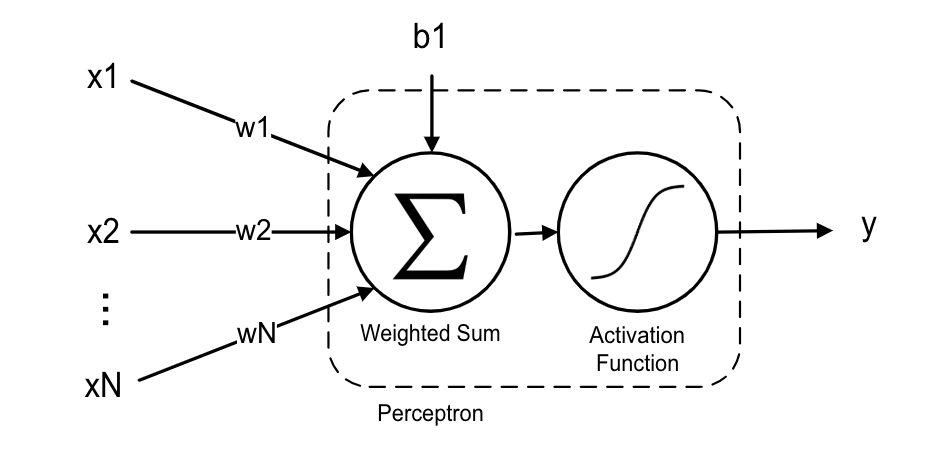
\includegraphics[width=0.6\textwidth]{Images/perceptron.png}
\caption{Perceptron architecture and basic neural network building block.}
\label{fig:perceptron}
\end{figure}

\begin{figure}[htbp]
\centering
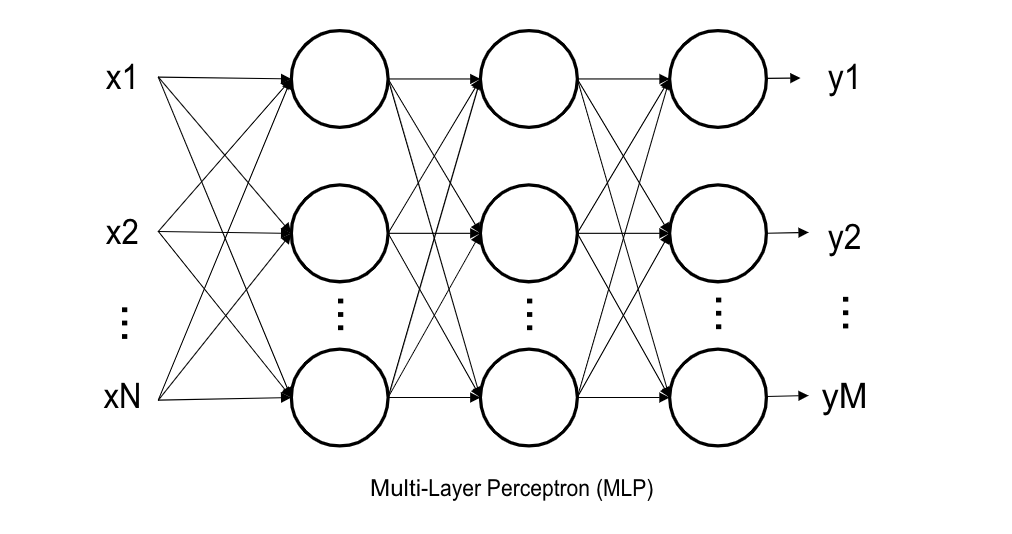
\includegraphics[width=0.6\textwidth]{Images/mlp.png}
\caption{Multi-layer perceptron architecture showing feedforward neural network structure.}
\label{fig:mlp}
\end{figure}

% #############################################################################
\section{Attention and Transformers}

Self-attention mechanisms, encoder-decoder architectures, and positional encoding.

\begin{figure}[htbp]
\centering
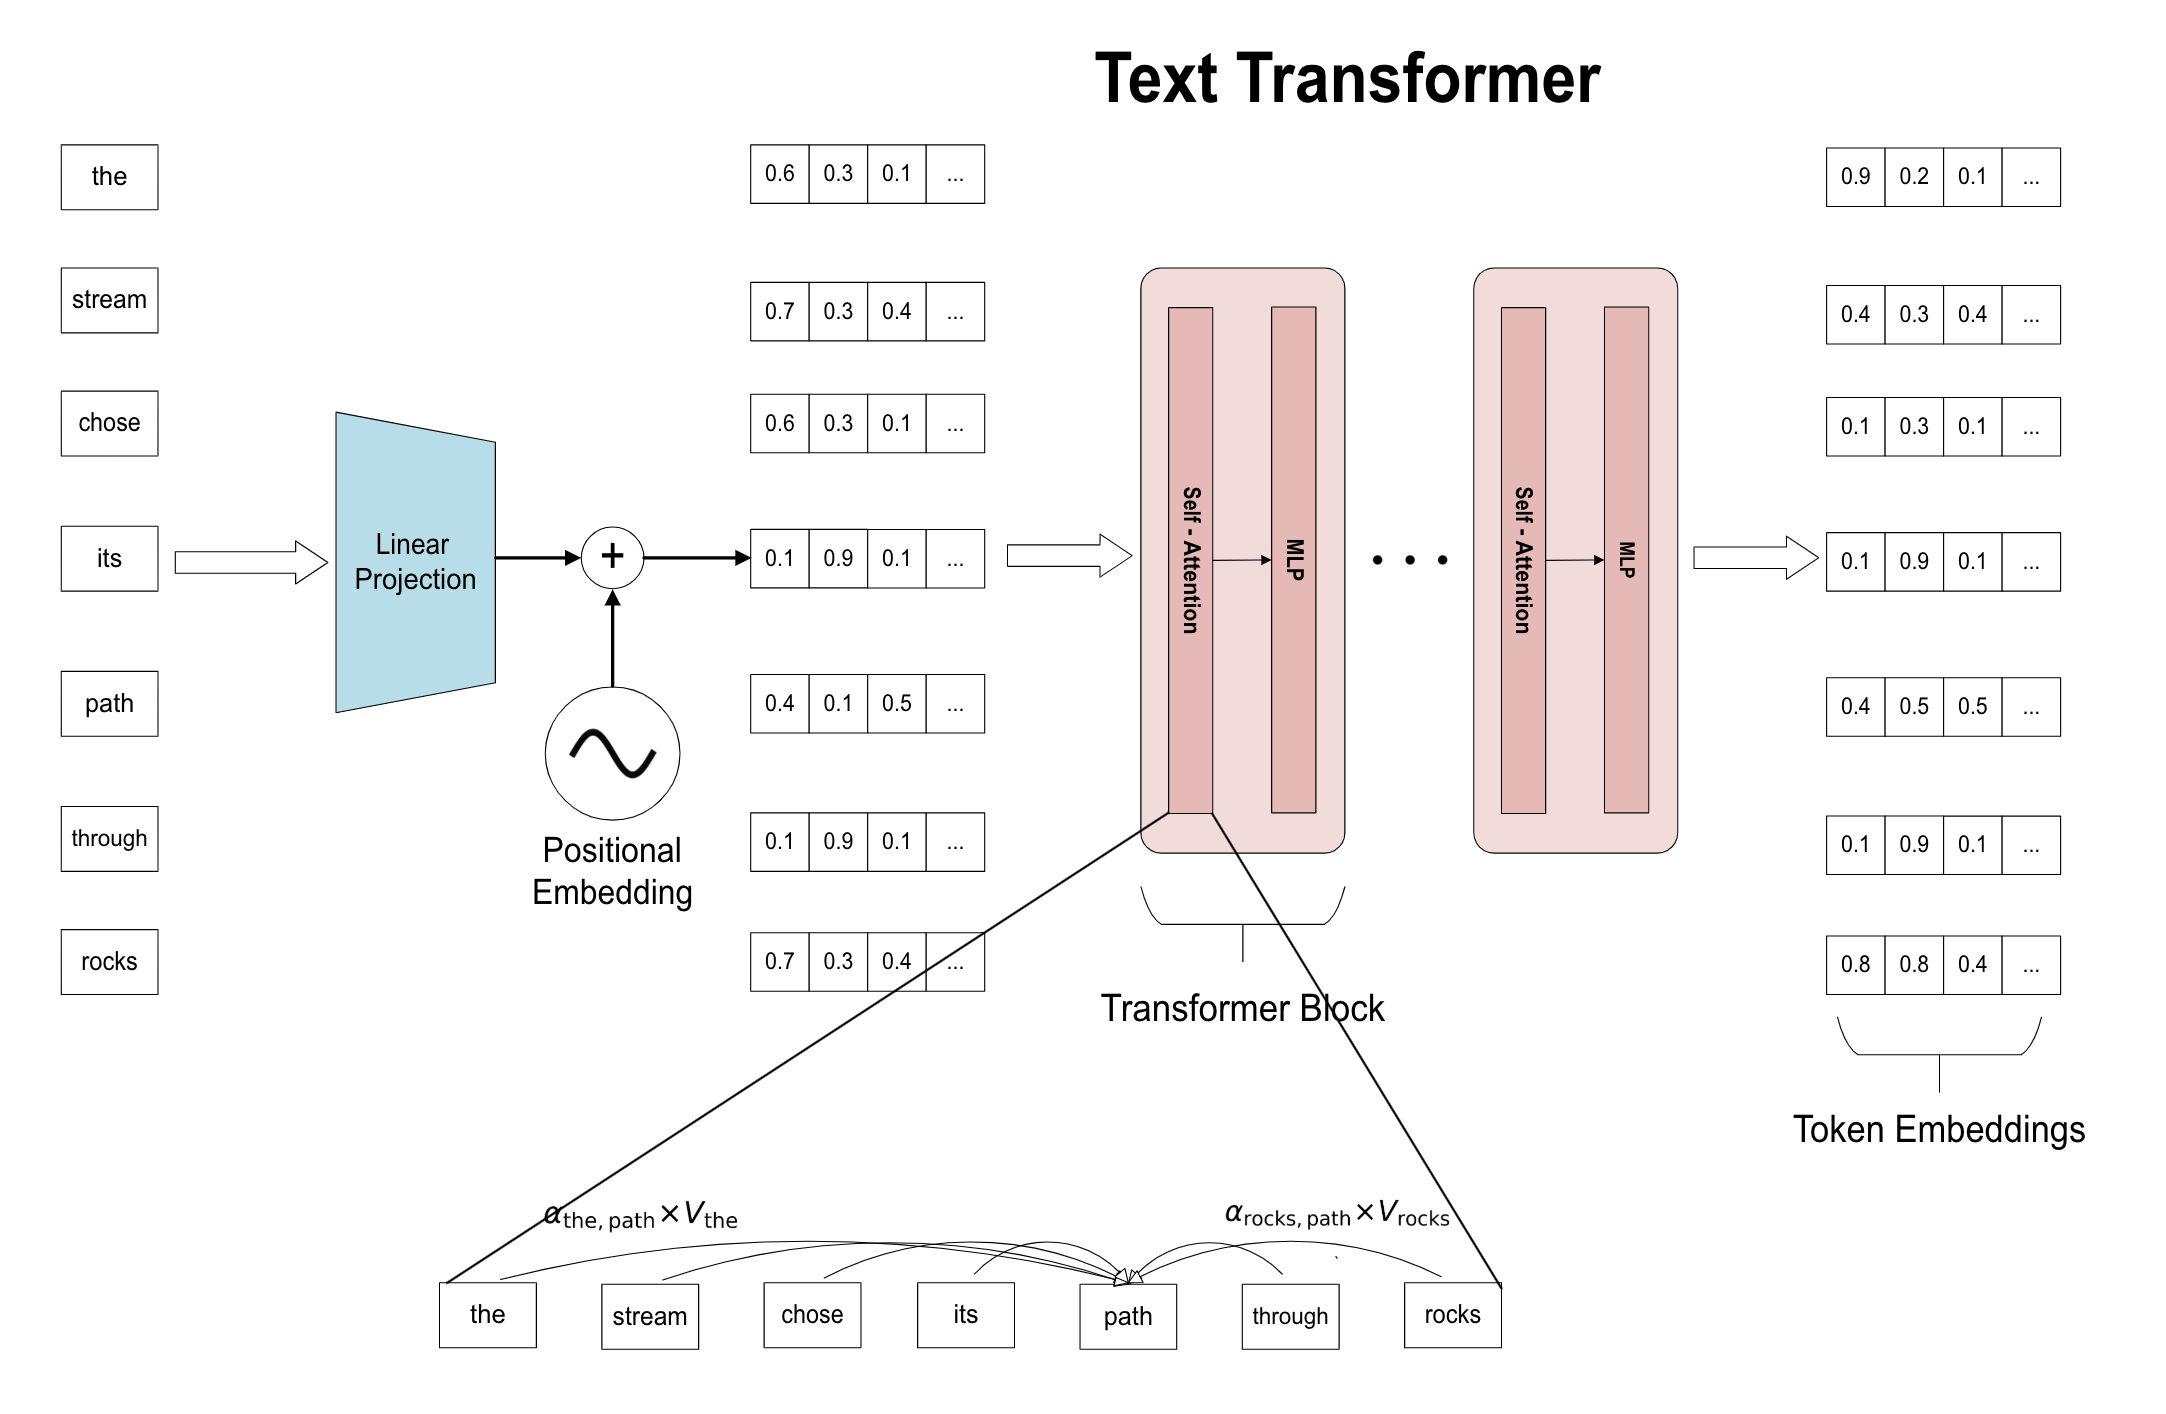
\includegraphics[width=0.8\textwidth]{Images/transformer.png}
\caption{Transformer architecture with self-attention mechanisms and encoder-decoder structure.}
\label{fig:transformer}
\end{figure}

% #############################################################################
\section{Transformers for Computer Vision}

Application of transformer architectures to computer vision tasks and visual understanding.

\begin{figure}[htbp]
\centering
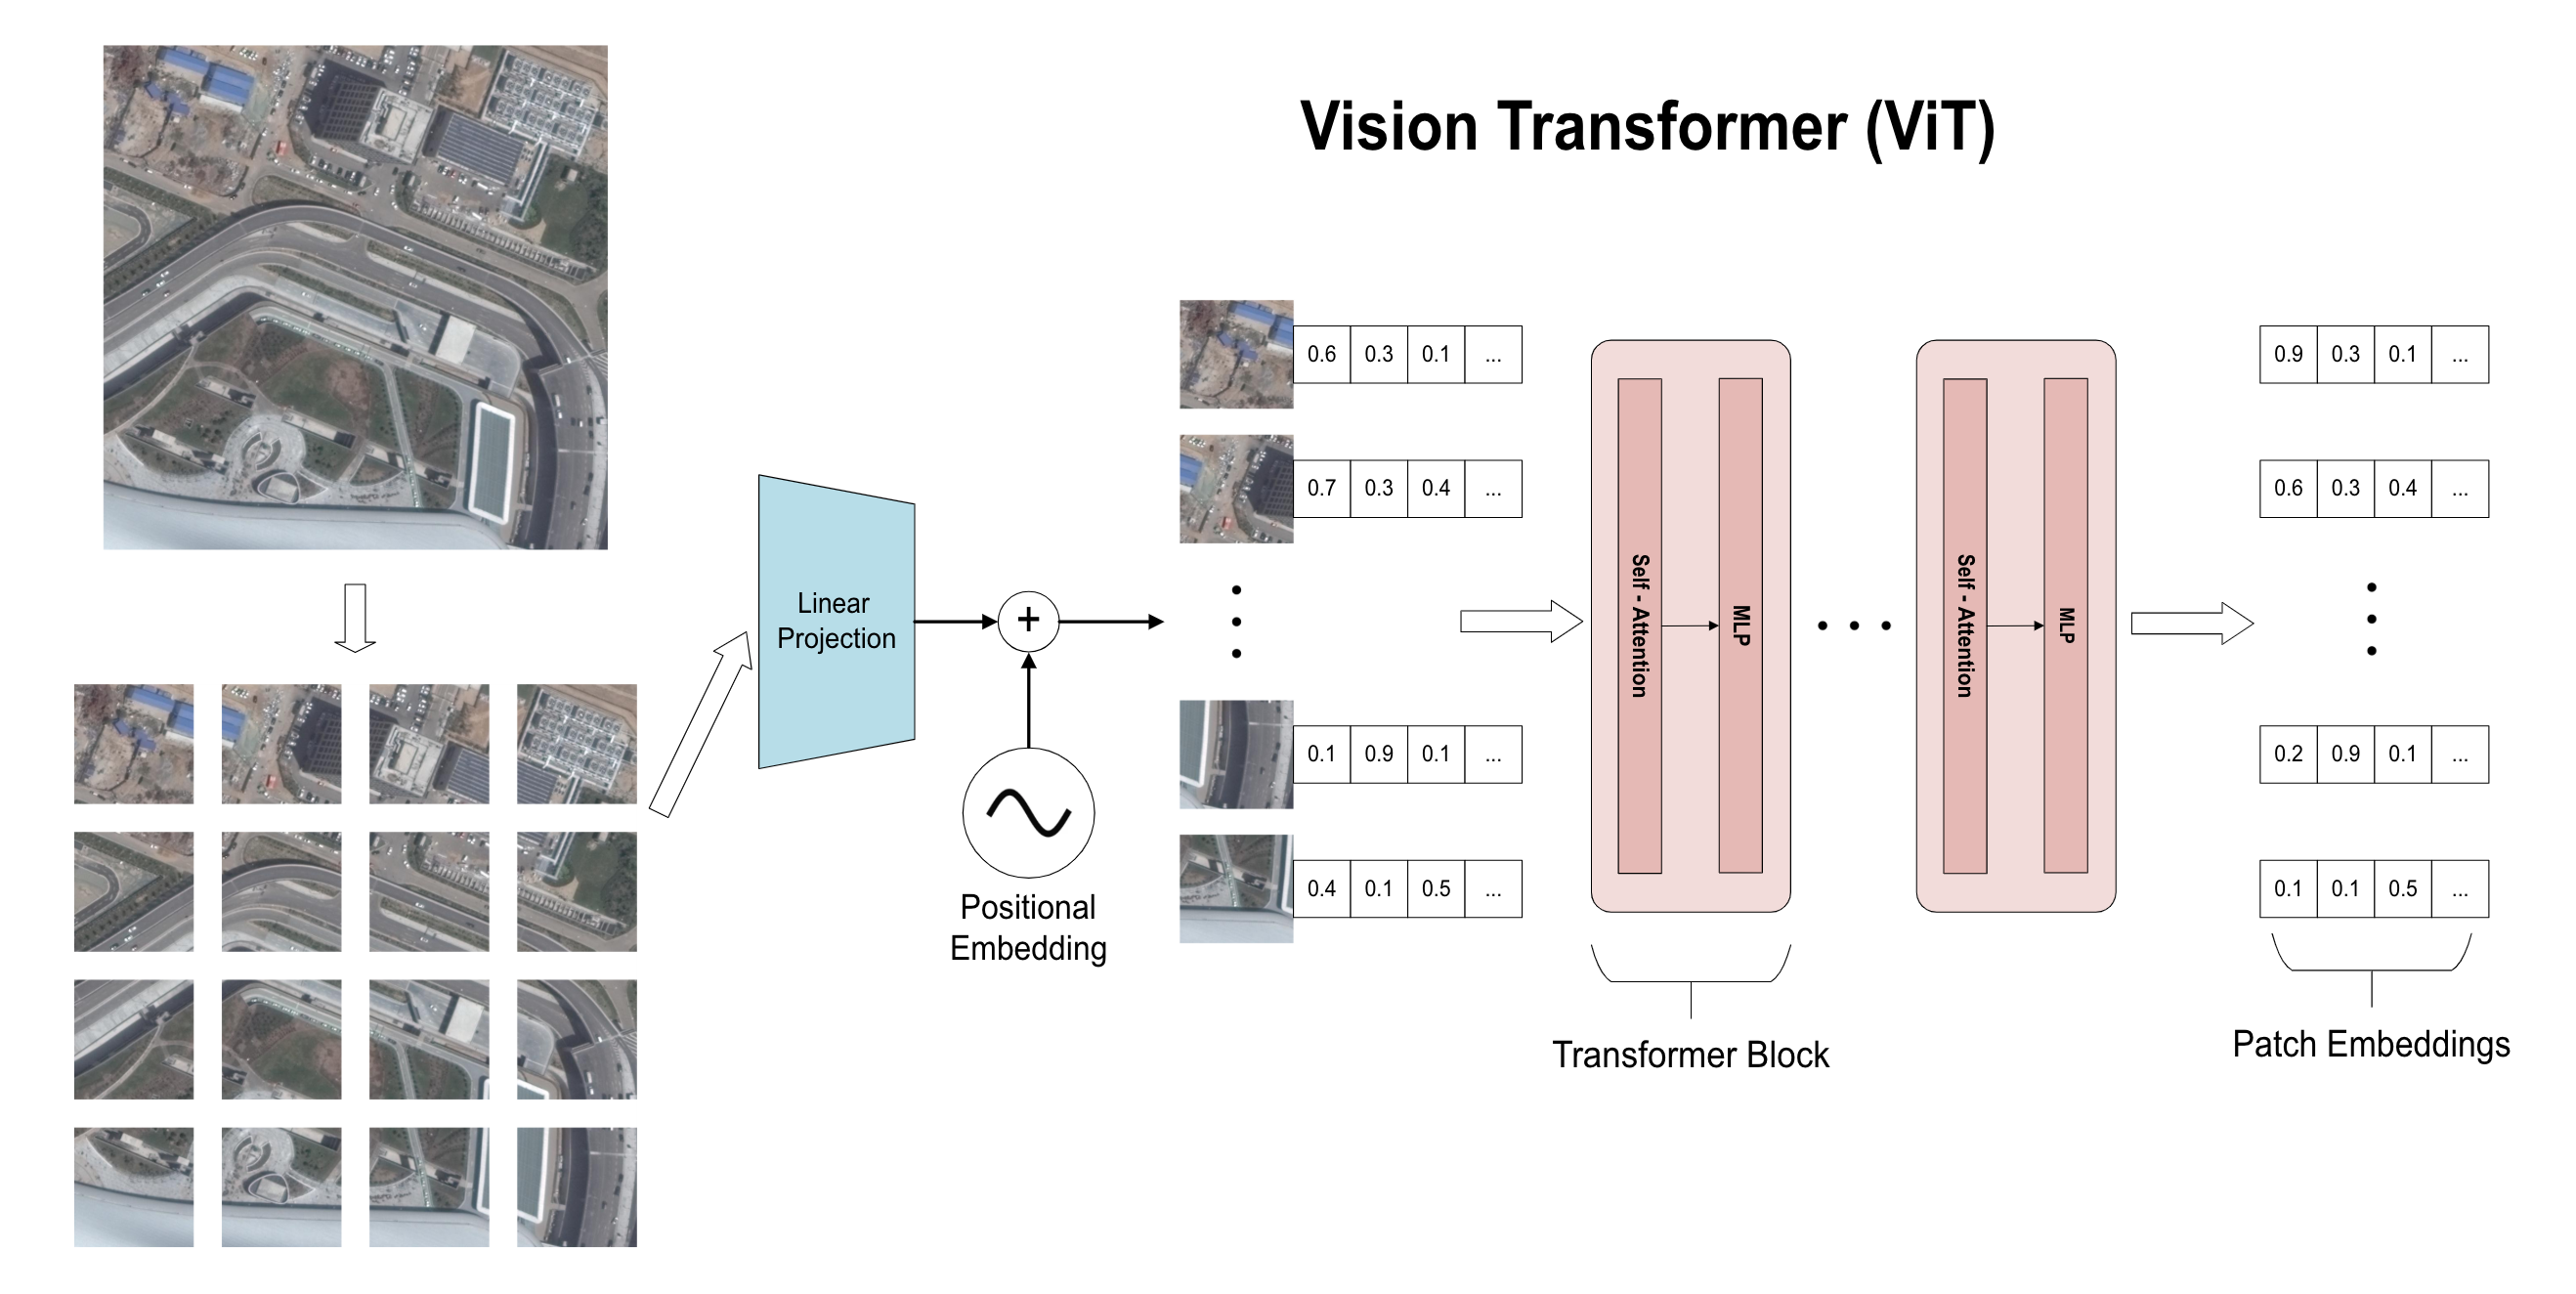
\includegraphics[width=0.8\textwidth]{Images/vit.png}
\caption{Vision Transformer (ViT) architecture for image classification and feature extraction.}
\label{fig:vit}
\end{figure}

% #############################################################################
\section{Image Segmentation}

Deep learning approaches for image segmentation tasks and methodologies.

\begin{figure}[htbp]
\centering
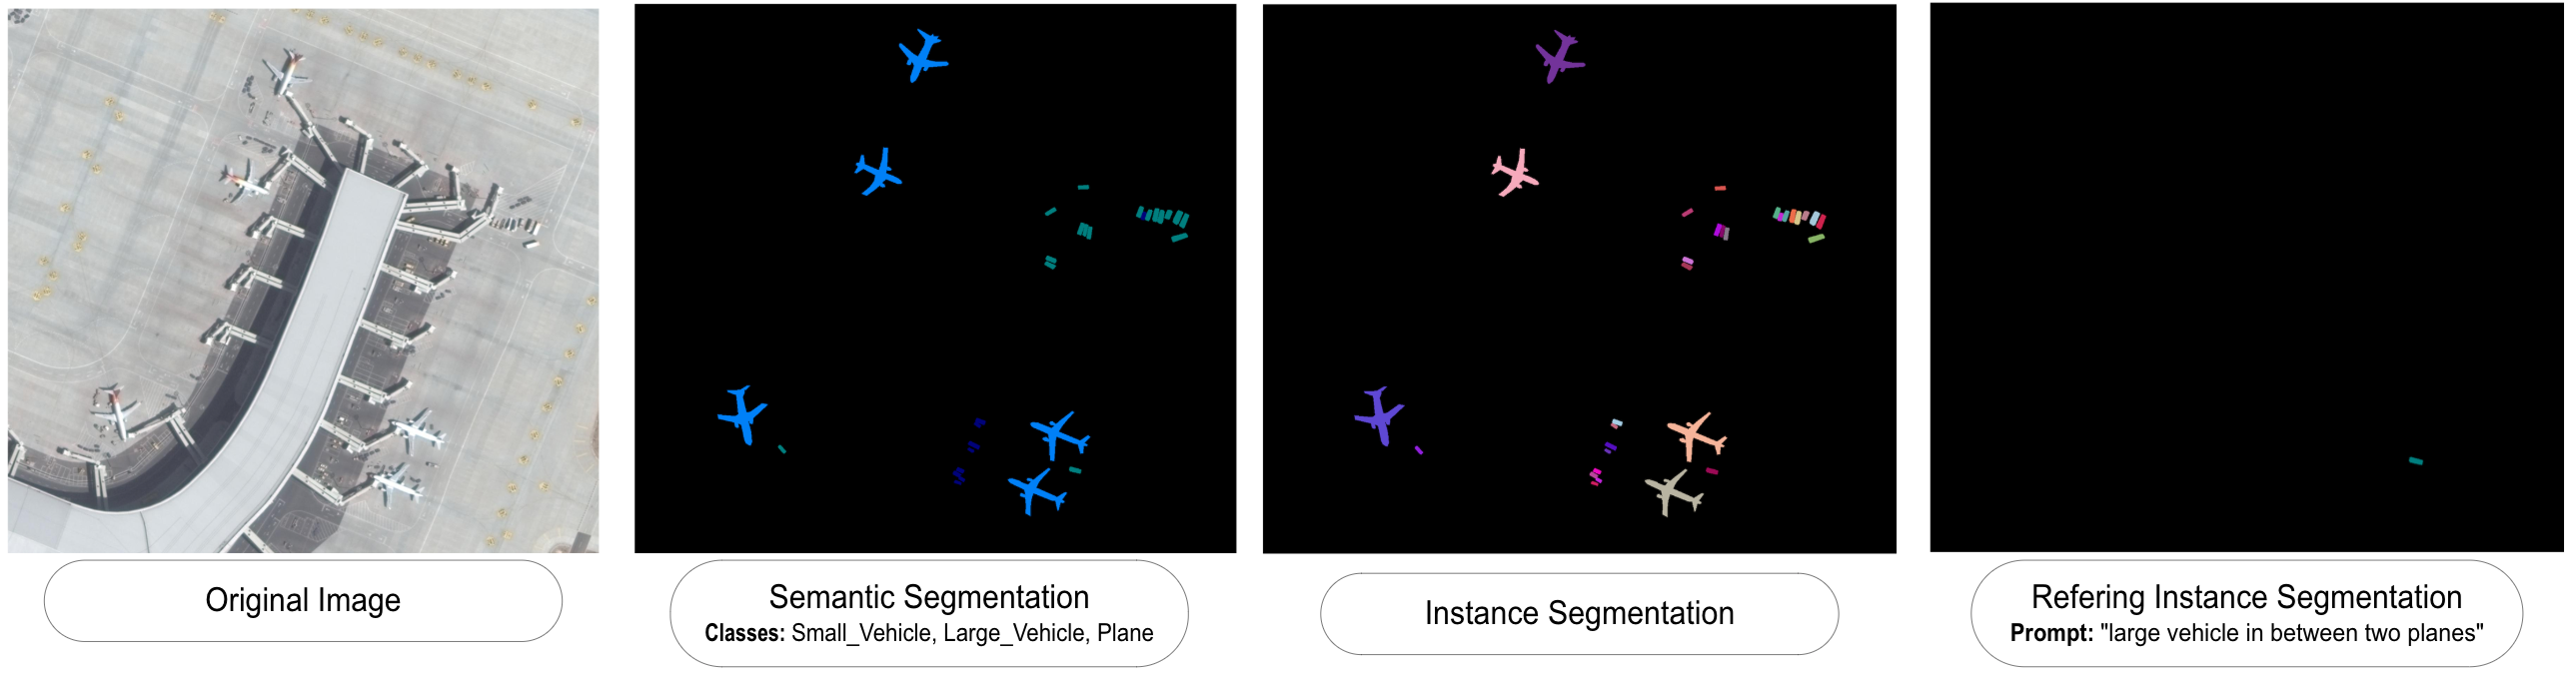
\includegraphics[width=1.0\textwidth]{Images/segmentation.png}
\caption{Comparison of segmentation types: semantic segmentation, instance segmentation, and referring instance segmentation with natural language prompts.}
\label{fig:segmentation}
\end{figure}

% #############################################################################
\section{Vision-Language Models}

Multimodal architectures that process both visual and textual information.

\subsection{CLIP and Visual-Language Learning}

Contrastive Language-Image Pre-training model architecture and visual-language learning methodologies.

\begin{figure}[htbp]
\centering
\subfigure[Contrastive pre-training methodology.]{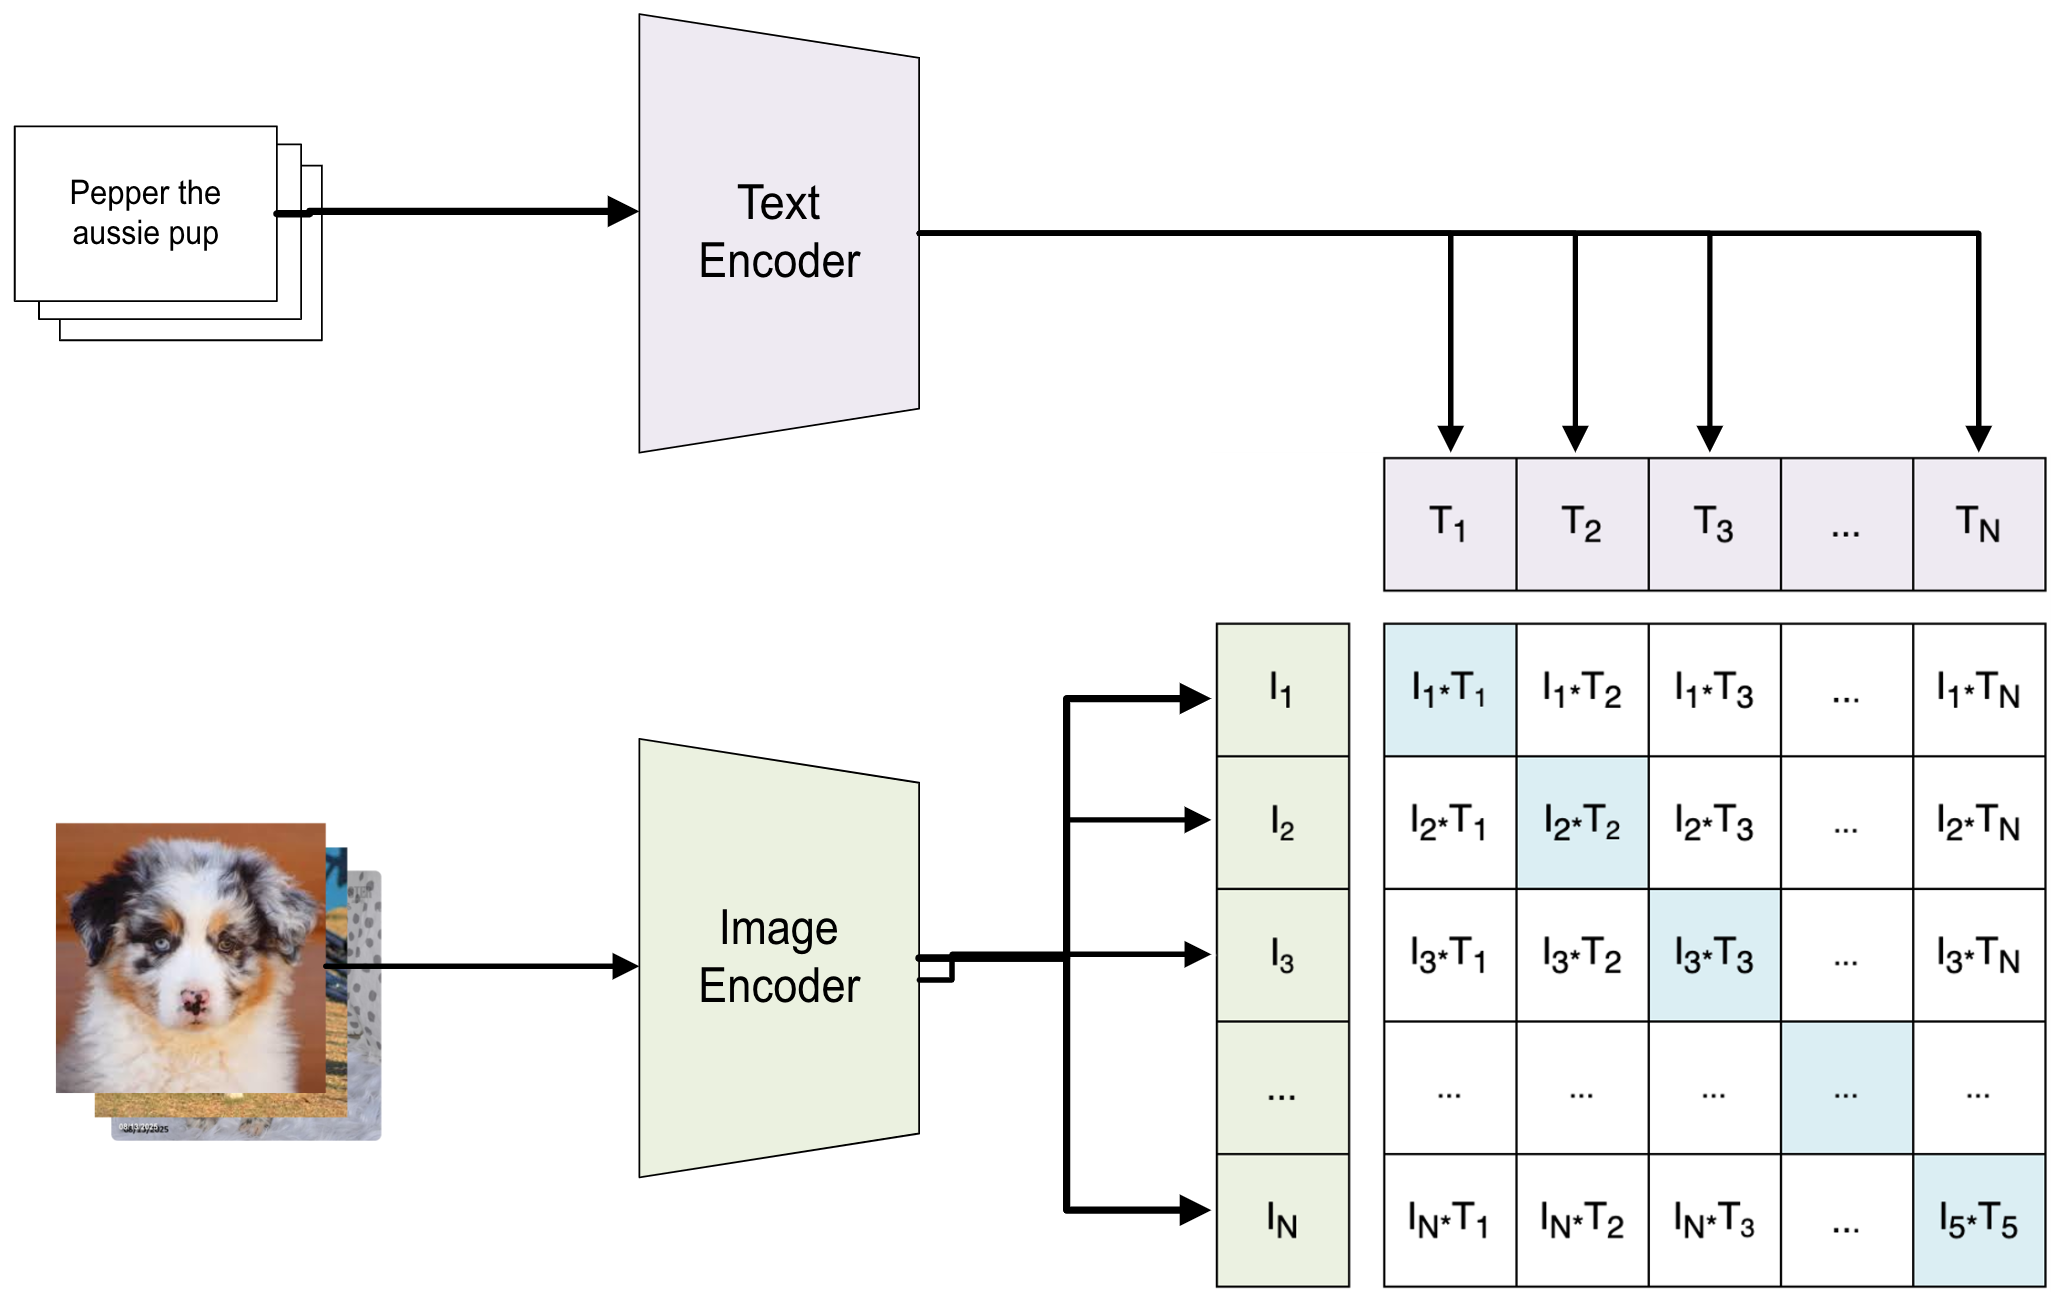
\includegraphics[width=0.45\textwidth]{Images/contrastive_pretraining.png}\label{fig:contrastive_pretraining}}
\hfill
\subfigure[Zero-shot prediction capabilities.]{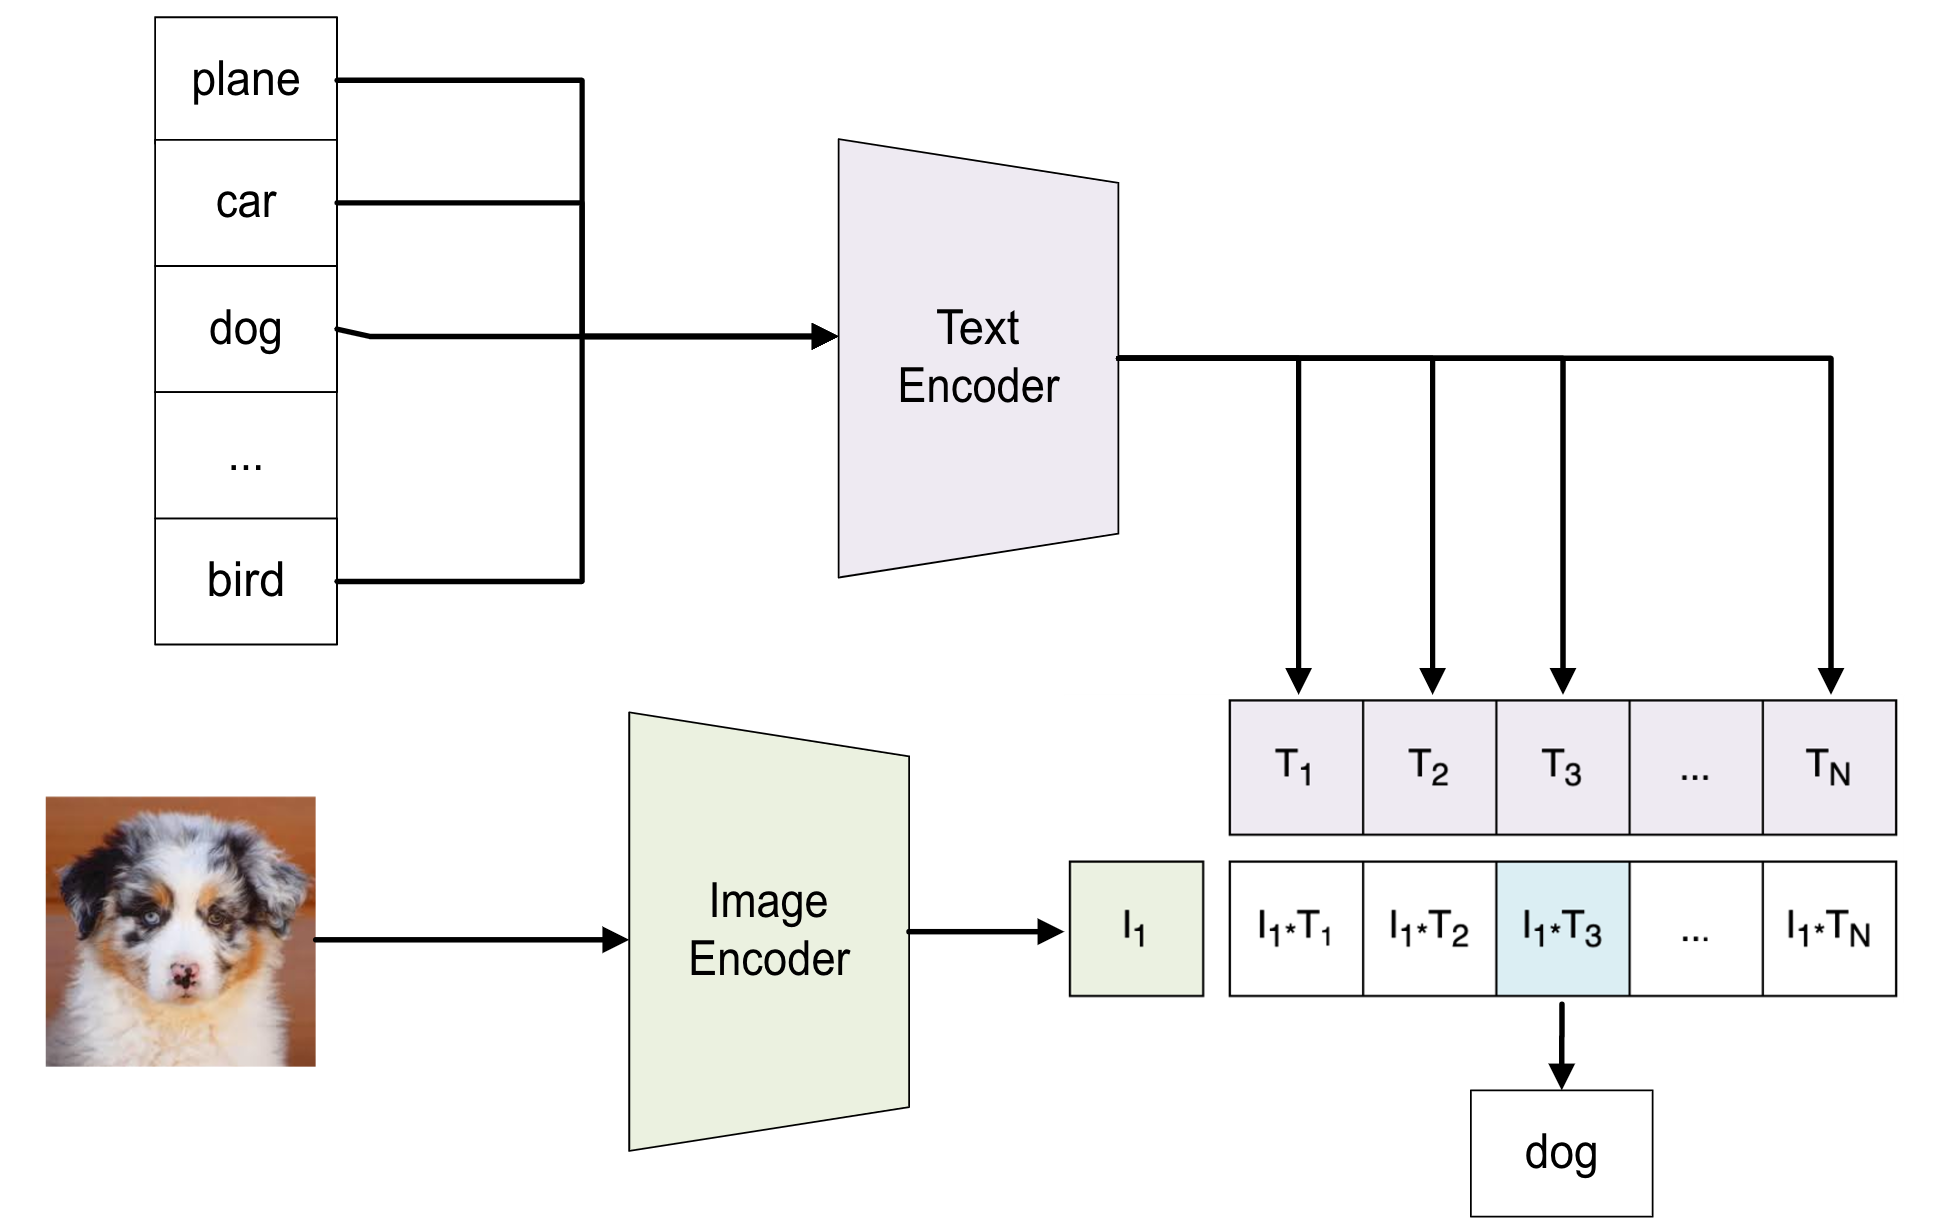
\includegraphics[width=0.45\textwidth]{Images/zero_shot_prediction.png}\label{fig:zero_shot_prediction}}
\caption{CLIP architecture components showing contrastive pre-training and zero-shot prediction mechanisms.}
\label{fig:clip_architecture}
\end{figure}

\subsection{Large Language Models}

Foundation models for natural language understanding and generation in multimodal contexts.

\begin{figure}[htbp]
\centering
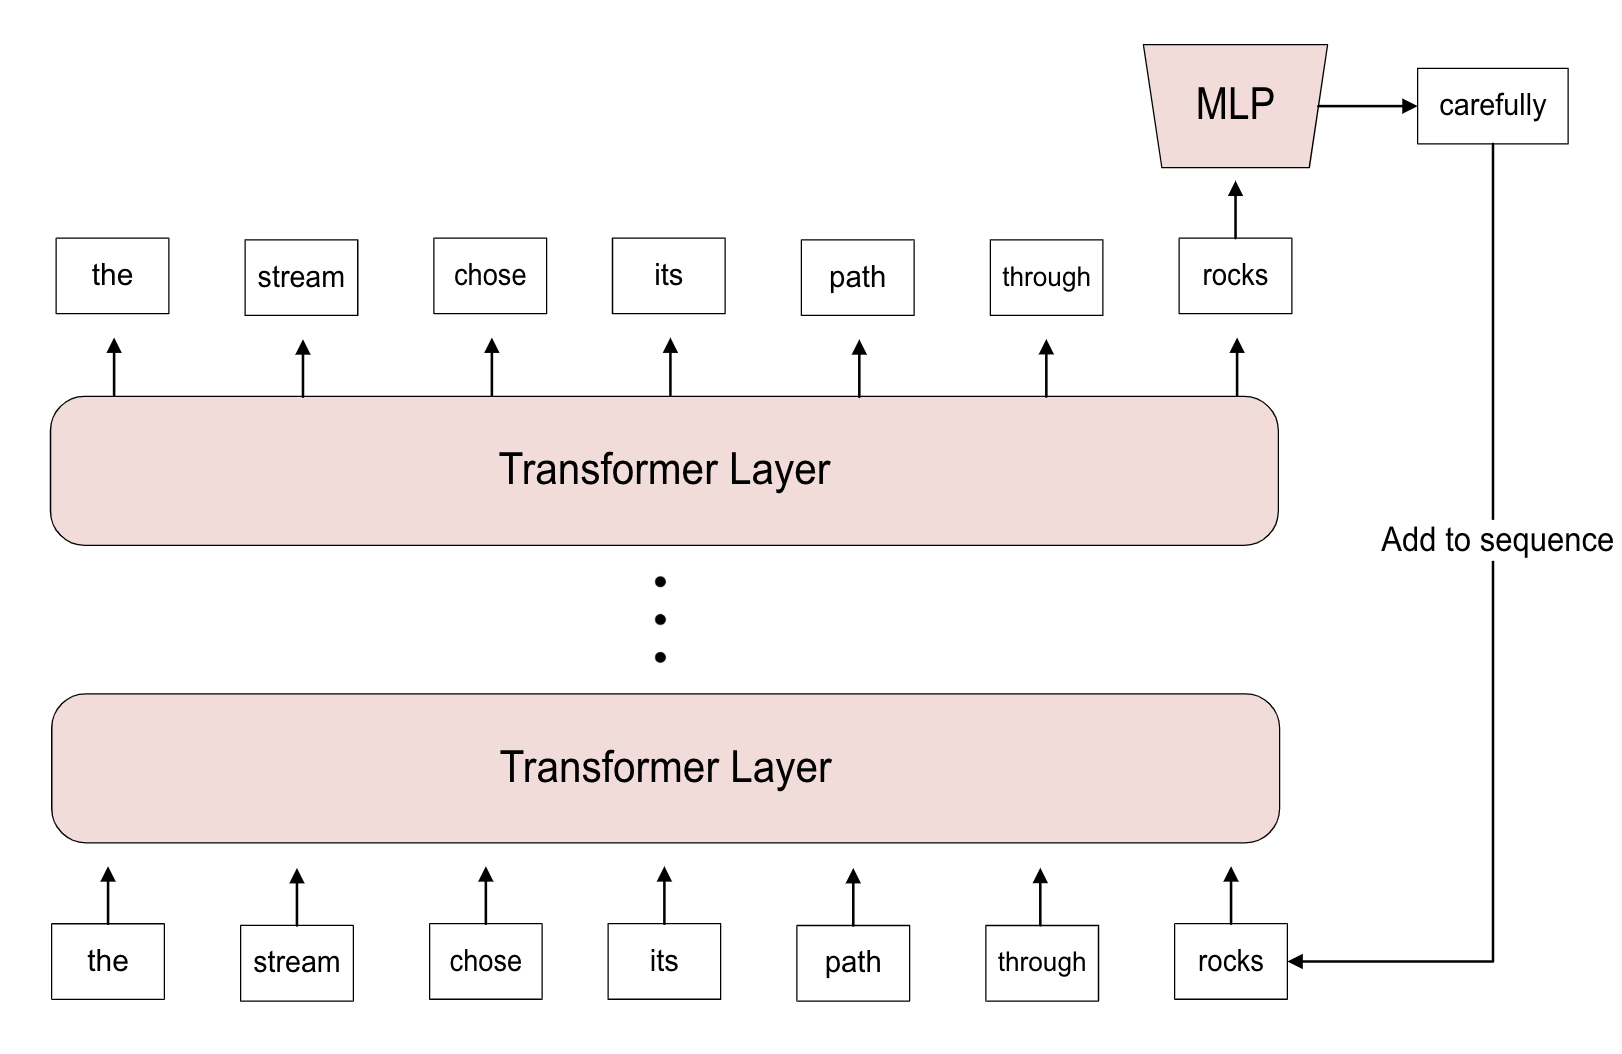
\includegraphics[width=0.8\textwidth]{Images/gpt.png}
\caption{GPT autoregressive language model architecture showing the transformer decoder stack with next-token prediction and feedback mechanism.}
\label{fig:gpt}
\end{figure}